\documentclass[10pt]{article}
\usepackage{color}
\usepackage{tikz}

% Tikz settings optimized for causal graphs.
% Just copy-paste this part
\usetikzlibrary{shapes,decorations,arrows,calc,arrows.meta,fit,positioning}
\tikzset{
    -Latex,auto,node distance =1 cm and 1 cm,semithick,
    state/.style ={ellipse, draw, minimum width = 0.7 cm},
    point/.style = {circle, draw, inner sep=0.04cm,fill, node contents={}},
    bidirected/.style={Latex-Latex,dashed},
    el/.style = {inner sep=2pt, align=left, sloped},
    %circle/.style = {circle, draw, inner sep=0.04cm, hollow, node contents={}} 
}

\begin{document}

% The graph
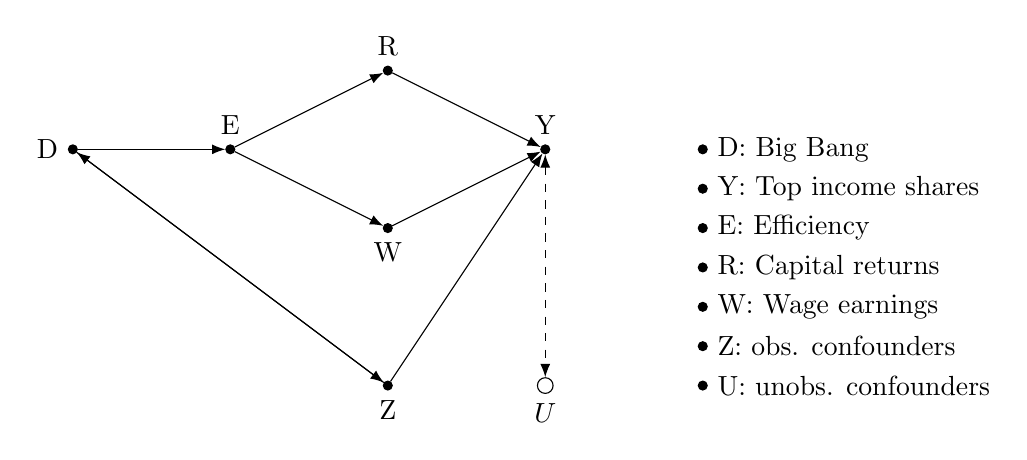
\begin{tikzpicture}

\tikzstyle{h}=[circle,draw, inner sep=2]
    % X and Y nodes
    \node (d) at (-2,0) [label=left:D, point];
    \node (e) at (0,0) [label=above:E, point];
	\node (r) at (2,1) [label=above:R, point];
	\node (w) at (2,-1) [label=below:W, point];
	%\node (i) at (0,-2.5) [label=below:I, point];
	%\node (s) at (0,-2.5) [label=below:S, point];  
	\node (y) at (4,0) [label=above:Y, point];
	\node (z) at (2,-3) [label=below:Z,point];
	%\node (w) at (2,1.5) [label=above:W,point];
	%\node[circle] {Circle};
	%\draw  node[circle]{} (2,-1.5);
	%\draw  node[fill,circle,inner sep=0pt,minimum size=1pt] {}
	\node[h, label=below:$U$] (u) at (4, -3){};
		%LEGEND:
	\node (a) at (6,0) [label=right:D: Big Bang, point];
	\node (b) at (6,-0.5) [label=right:Y: Top income shares, point];
	\node (c) at (6,-1) [label=right:E: Efficiency, point];
	\node (f) at (6,-1.5) [label=right:R: Capital returns, point];
	\node (k) at (6,-2) [label=right:W: Wage earnings, point];
	\node (h) at (6,-2.5) [label=right:Z: obs. confounders, point];
	\node (i) at (6,-3) [label=right:U: unobs. confounders, point];
	
    % Directed edge
    \path (d) edge (e);
    \path (d) edge (z);
    \path (e) edge (r);
    \path (e) edge (w);
    \path (z) edge (d);
    \path (z) edge (y);
    \path (w) edge (y);
    \path (r) edge (y);
    
    
    % Bidirected edge
    %\path[bidirected] (d) edge[left=60] (u);
    \path[bidirected] (y) edge[left=60] (u);
	%\path[bidirected] (i) edge[left=60] (y);
	%\path[bidirected] (s) edge[left=60] (d);
	%\path[bidirected] (s) edge[left=60] (i);
	%\path[bidirected] (z) edge[left=60] (y);

\end{tikzpicture}

\end{document}

